\chapter{$K_S^0$ Reconstruction Study}

The final states of $B^0 \to K_S^0  K_S^0  K_S^0 $ only depends on the decay of $K_S^0$. The main decay channels of $K_S^0$ is to either $\pi^+ \pi^-$ at branching fraction of about 0.692, or to $\pi^0 \pi^0$ at branching fraction of 0.307. The characteristics of these two decays are much different in terms of the response from Belle II detector. The charged decay that yields  $\pi^+ \pi^-$ leaves two tracks (track as data object) originating from VXD or CDC volumes with opposite charge. While the $\pi^0$ main decay channel is $\pi^0 \to \gamma \gamma$. This creates a bunch of clusters on ECL (ECLClusters as data object). The reconstruction of the decay channel is performed through  $\pi^+ \pi^-$. There are mainly two reasons for not selecting $\pi^0$ as final states.
 Firstly, $\pi^0 \to \gamma \gamma$ comes with a big load of background as fake $K_S^0$. The reconstruction of ECLClusters provides no constrain on $K_S^0$ vertex so it's almost impossible to suppress the combination background using vertexing quality in this case. The only reliable selection will be the mass of $K_S^0$ which typically varied around its nominal mass with a few hundred of keV. 
 The $\gamma$ however, could be originating from many other resource, such as beam background, and charged track radiation. Using mass window of $K_S^0$ could not effectively reject the noticeable fraction of fake rate. The MC study shows the fraction of true $K_S^0$ among all accepted candidates using mass cut only is about 3\% using 2 neutral pions.  Secondly, with $K_S^0$ from neutral pions  included, the events of $B^0$ that consist of one or more such $K_S^0$ will have poorly reconstructed vertices. The precise measurement of time-dependent \textit{CP} violation emphasizes vertexing quality. Even with $B^0 \to K_S^0  K_S^0  K_S^0 $ that only uses charged pions for final states, it already has no primary vertex from $B^0$ which leads to the worse resolution of vertex position compared to the channel like $B^0 \to J/\psi K_S^0$, which has two direct charged tracks of $e^+e^-$ or $\mu^+ \mu^-$  because of the very short flight distance of $J/\psi$. If one or more of $K^0_S$ has bad vertexing quality from its decay products, it will further reduce the precision of vertexing of $B^0$. This leads to a large uncertainties in defining the decay time of signal $B^0$ so as to the decay time difference which is the key observable to TDCPV measurement. Based on above, we only reconstruct $K_S^0$ from its charged decay products to improve the vertexing quality of $B^0$.
 
 \section{Cut-based $K_S^0$ Reconstruction}
 The $K_S^0$ has average life time at $(8.954 \pm 0.004) \times 10 ^{-11}s$ so the flight length of $K_S^0$ before it decays could be compared with the scale of detector size. In the typical Belle II energy scale, $K_S^0$ mainly decays inside of VXD volume, which covers from a few micrometer inside first layer of PXD, to the even outside of last layer of SVD ladder that is placed at 14cm away from the interaction point(IP). The flight length of $K_S^0$ from $B^0$ generic decay and $B^0 \to K_S^0  K_S^0  K_S^0 $ are shown in Fig 3-1 from MC13: 
 
 \begin{figure}[htpb]
 	\centering 
 	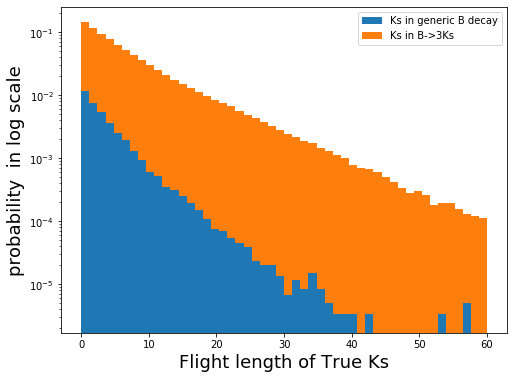
\includegraphics[height=8cm]{KsFlightLength}
 	\caption{Flight length of $K_S^0$ from MC, Blue is from generic $B^0$ decay and  orange is from $B^0 \to K_S^0  K_S^0  K_S^0$. Both are from MC13.}
 \end{figure}
 
 Due to the different topology of $B^0$ decay, the average momentum of $K_S^0$ in generic decay is smaller than the ones from generic $B^0$ decay, as well as the average flight length. It's clear that the fraction of $K_S^0$ decaying outside the IP is majority and there's no reason to constrain the origin of $K_S^0$ decay vertex to IP. So the basic cut-based reconstruction of $K_S^0$ is performed by the selection of invariant mass from its decay products then putting requirements on its vertexing fit quality without geometric constrain. The cu-based selection of $K_S^0$ is done by using BASF2 ``stdKshort:merged" list. In this ``stdKshort:merged" list, we first take all the ``V0" objects from BASF2 which use 2 online reconstructed charged tracks with opposite charge and a converged fitted vertex. The invariant mass between $0.45 < M < 0.55$ GeV is applied, where M is calculated from daughters' 4-vector. Then the reconstruction of $K_S^0$ is also performed by offline reconstruction using BASF2 which loads all tracks as charged pions and also requires the invariant mass between $0.45 < M < 0.55$ GeV and a converged fitted vertex. In both cases, the vertex fit is performed using TreeFit. The reconstruction efficiency $B^0$ is highly sensitive to the efficiency of charged pions, so we use charged pions with no extra cuts but only the M and converged vertex. Compared the $K_S^0$ from V0 and offline reconstructions, we can remove the duplicated $K_S^0$ when the two pions are from two same tracks, to form the $K_S^0$ candidates that still have many fake ones, see Fig 3-2.
 
 
 \begin{table}[htbp]
 	\centering
 	\large
 	\caption{Pre-selection criteria of $\pi^+ \pi^-$}
 	\begin{tabular}{c c c c }
 		\toprule
 		Selection & $\theta$ & CDC Hits Number & PID  \\
 		\hline
 		Criteria  & CDC acceptance &  $>20$ & pionID $> 0.1$\\
 		\bottomrule
 	\end{tabular}
 \end{table}


\begin{figure}[htpb]
	\centering 
	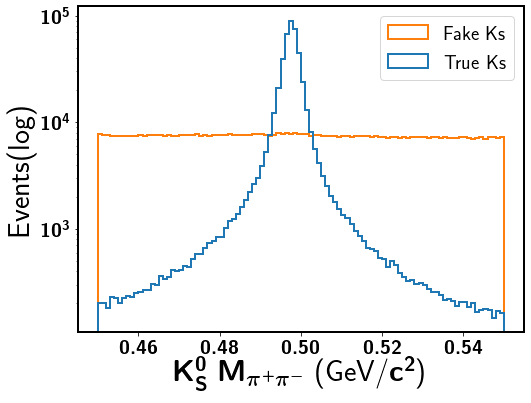
\includegraphics[height=8cm]{Ks_M}
	\caption{The distribution of invariant mass of $K_S^0$ candidates, blue line is the MC truth matched $K_S^0$ and the orange is the fake $K_S^0$ passing the selection.}
\end{figure}
The $K_S^0$ candidates from ``stdKshort:merged" is the default way to obtain $K_S^0$ in BASF2, 
however, the limitation of this cut-based $K_S^0$ reconstruction is the pollution from fake $K_S^0$. When using these $K_S^0$ candidates to reconstruct $B^0 \to K_S^0  K_S^0  K_S^0$, each of the fake $K_S^0$ has the chance to propagate to form a fake $B^0$ since $K_S^0$ is only intermediate states in this channel. This creates high fake rates in $B^0$ candidates and costs a large extra processing time for computing the kinematics and vertex fit of $B^0$ which could've been avoid. Even by then, the number of combinatorial backgrounds in $B^0$ from 3$K_S^0$ is still high. Thus, a multi-variate analysis (MVA) based $K_S^0$ identification package is developed.

\section{MVA-based $K_S^0$ Identification: KsFinder}

\subsection{Experience from Belle}
In order to improve the reconstruction performance of $K_S^0$, a multi-variate analysis based (MVA-based) package called KsFinder has been developed. The reconstruction of $K_S^0$ can be treated as a typical classification problem. The input is a set of observable that describes the characteristics of $K_S^0 \to \pi^+ \pi^-$ decay. The targeted output is the signal or background flag from the MC truth-matching called ``isSignal" where isSignal = 1 (0) stands for being a true(fake) $K_S^0$. From the experience of Belle, the $K_S^0$ reconstruction was first done by using cut-based method to select primary candidates, then MVA-based classifier was implemented by assigning two likelihood indicators to each $K_S^0$ candidates. The package used by Belle is called ``nisKsFinder"\cite{b2book}. It classifiers the two likelihood variables based on NeuroBayes algorithm, which defines the goodness of $K_S^0$. A good candidate from ``nisKsFinder" is the one with low likelihood of being $\Lambda$ particle and the high likelihood of being a V0-like particle. The two variables used here are called ``nb\_nolam" and ``nb\_vlike". By putting cuts on these two variables, a purification of $K_S^0$ can be made. 

%\begin{figure}[htpb]
%	\centering 
%	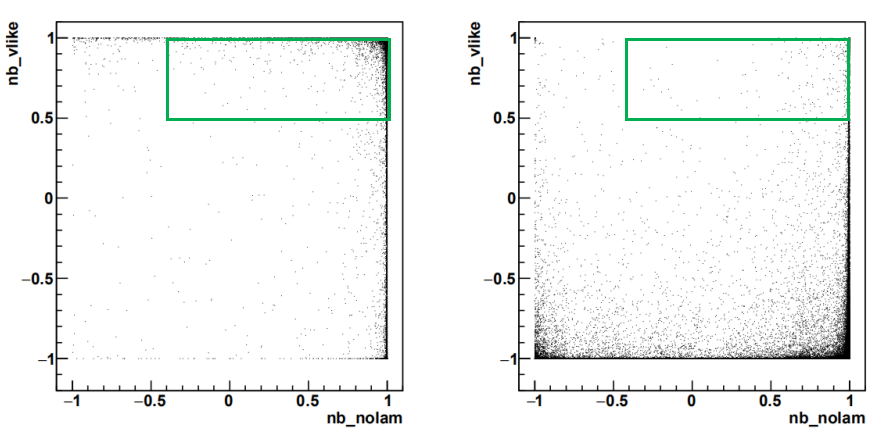
\includegraphics[height=7.5cm]{nisksfinder}
%	\caption{The lefe plot shows the output from nisKsFinder of true $K_S^0$, and the right one shows that of fake $K_S^0$.}
%\end{figure}

\subsection{FastBDT algorithm}
In Belle II, such tool is of missing from the current BASF2 framework. Since ``NeuroBayes" algorithm is a third-party commercial product and is not being supported by its producer, the usage and maintenance of it could face unexpected issue with no warranty of fixing ensured. So it's not going to be the default option for $K_S^0$ classification in Belle II. Instead,  stochastic gradient-boosted decision trees are widely employed for multivariate classification and regression tasks in modern high energy physics field. Particularly, a speed-optimized and cache-friendly
implementation for MVA classification called FastBDT (FBDT) is popularly used. Compared to other popular classification algorithm in software framework, such as TMVA, scikit-learn and XGBoost, FastBDT method is proven to be one order of magnitude faster during the fitting  and applying phase. 

A general DT (decision tree) performs classification using a number of consecutive cuts. The maximum number of cuts are called ``depth of tree" and it's a hyper-parameter of DT. For each data point, there are known labels called ``feature" and data points passing the previous cuts on one feature are sent to the next label. At each nodes, a cumulative probability histogram can be defined by counting the signal and background regarding a certain label. A gain presenting the separation power at each node is calculated using all possible labels. The cut on that label is determined by making a maximum of gain. This process locally maximizes the separation of signal and background at each node. At the end layer of tree, which is called ``terminal nodes" of tree, the whole data set are spitted into different groups by DT. In each group, a fraction of signal is calculated using all data points in the group. Such process is illustrated as Fig 3-4. 

\begin{figure}[htpb]
	\centering 
	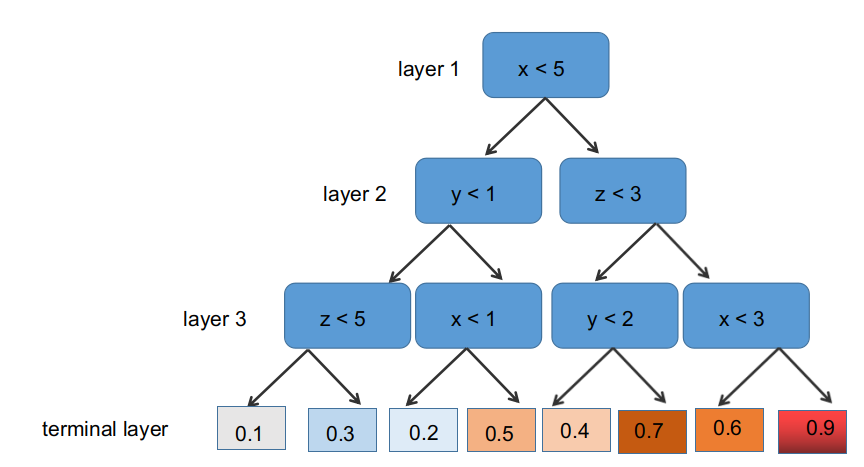
\includegraphics[height=8cm]{DT}
	\caption{Basic structure of a DT with depth = 3 and label of x,y,z. The last layer is terminal node and the number is signal fraction. The number (color demonstrated) is the signal fraction of data points in the nodes}
\end{figure}

The mathematical idea behind this method is to treat the data points as a data set defined on a multi-dimension hyper-space. As long as the signal/background data points show certain concentration in a sub-region of the hyper-space, it's possible to locally increase the signal fraction by consecutively cutting on the edge where signal and background separate. The cut on labels at each node is the edge of the sub-region. The deeper a DT is, the more edges of the hyper-space will be cut. So if a DT has too many layers (too deep), the data points in the sub-region can achieve a over-fitted signal fraction and won't represent a true distribution of whole data set because of the statistical fluctuation in the small sub-region. As a result, the classifier is over-fitted and performs poorly on new data points. There are pruning algorithms which automatically remove cuts prone to over-fitting
from the DT, details can be found here \cite{olshen1984classification}.

Avoiding the over-fitting of DT limits the depth of a tree strongly while a single shallow DT can only roughly separate signal and background. For a problem of $K_S^0$ classification, number of observables is much more than the usual tree depth (a few layers). So during the fitting phase, a sequence of many shallow DT is formed. For all the DTs, a negative binomial log-likelihood loss-function is minimized. The generation of DTs in this step is called ``Boost". Combining many weak-learners (single DT), a classifier with large separation power is constructed. The number of trees $N$ (or boosting steps) is the additional hyper-parameter of the model. 
The FastBDT implements a optimized algorithm from a derived Gradient BDT method (GBDT)\cite{friedman2001greedy} and gain an order of magnitude faster execution time. The comprehensive comparison between FastBDT and other popular methods in Belle II scope is described in here \cite{keck2016fastbdt}. 

\begin{figure}[htpb]
	\centering
	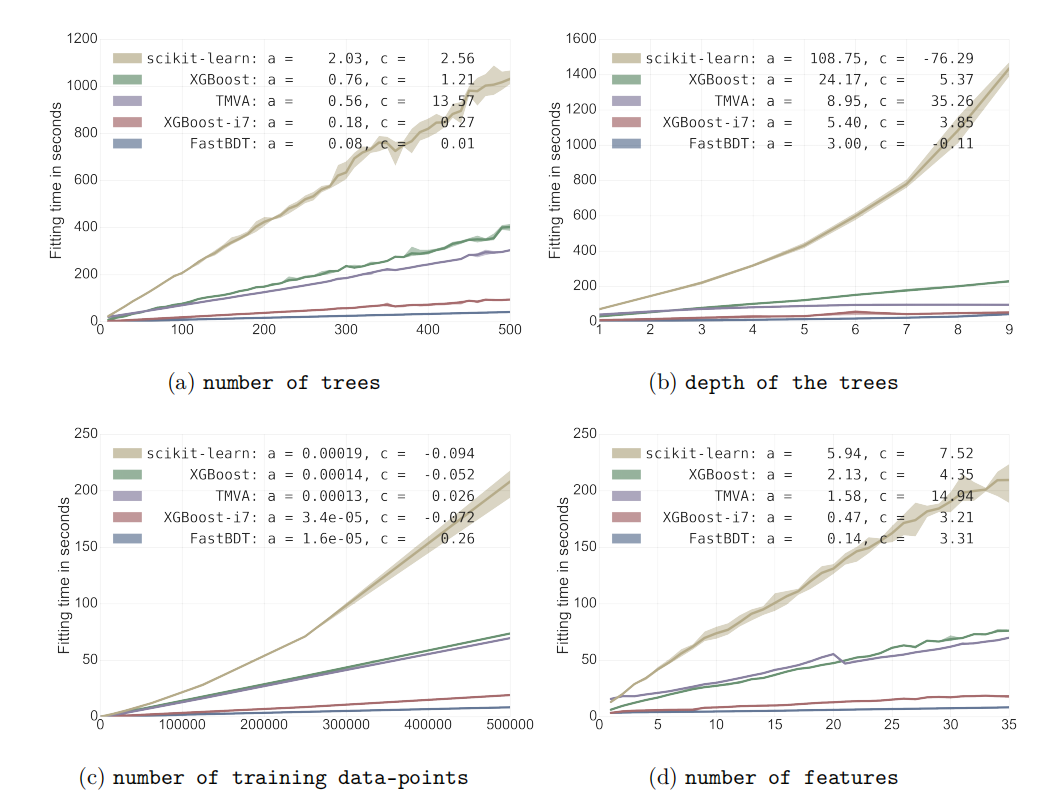
\includegraphics[height=12cm]{speedFBDT}
	\caption{Runtime in fitting phase with different hyper-parameters comparison among FastBDT and XGBT,TMVA,scikit-learn.\cite{keck2016fastbdt}}
\end{figure}

\subsection{Decay Topology of $K_S^0 \to \pi^+ \pi^-$}
The first step for developing $K_S^0$ MVA classification is to determine the input variables for FastBDT method which should represent the decay feature of $K_S^0$.
The remaining background of  $K_S^0 \to \pi^+ \pi^-$ after the cut-based reconstruction comes from different resources. In these resources, the main contributions are false combination of tracks, V0-like particle mis-identification, and looped tracks. 

The false combination of tracks includes two major cases. First is when one of the two daughter is $\pi^{+/-}$ and the other is not. This often happens when a charged pions from a neutral mother with a capability of decaying into multiple charged tracks, like $D^+ \to \mu^- \nu_{\mu} K^- \pi^+$. On the other hand, it's also possible that both of two tracks are correctly reconstructed from $\pi^{+/-}$ but they are not from the same mother, or the mother is not a $K_S^0$ particle due to the missing of other daughters, such as $D^+ \to K_S^0 (  \to \pi^+ \pi^-) \pi^+$. The decay shape resembled the above cases are illustrated as the following:  


\begin{figure}[htpb]
	\begin{minipage}[t]{0.5\linewidth} % 如果一行放2个图,用0.5,如果3个图,用0.33
		\centering 
		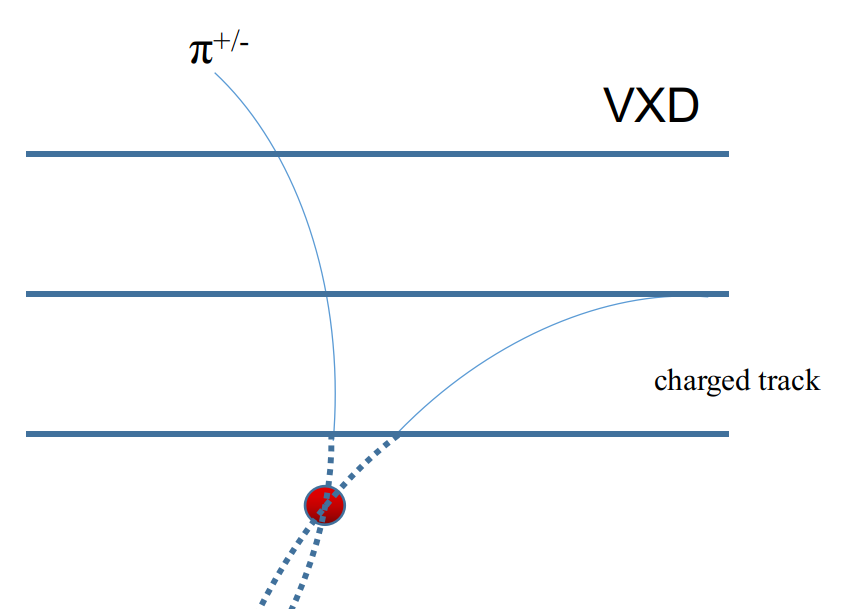
\includegraphics[width=7cm]{fakeks1} 
		\label{fig:side:a} 
	\end{minipage}%
	\begin{minipage}[t]{0.5\linewidth} 
		\centering 
		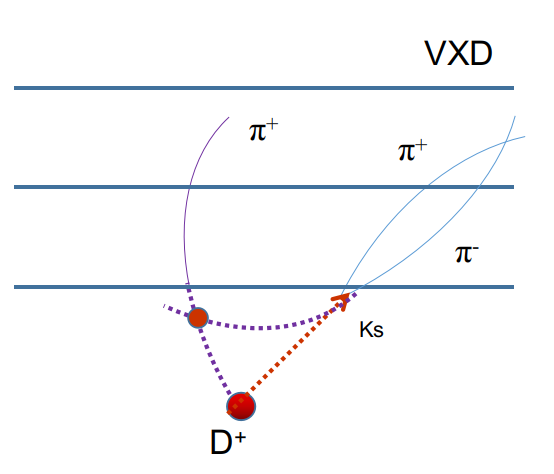
\includegraphics[width=7cm]{fakeks2} 
		%\caption{ } 
		\label{fig:side:b} 
	\end{minipage}% 
	
	\caption{The left shows the case when a charged track (not a pion) combined with a true pion as a fake $K_S^0$, the right shows the case when two daughters are correctly reconstructed as pion but not from the correct mother. }
\end{figure}

The V0-like particles mainly refer to $K_S^0$, $\Lambda$ and $\gamma$. $\gamma \to e^+ e^-$ yield is significantly lower than the previous two types and the mass different between pion and electron is very large, so the PID values can be used to well-distinguished them. As for the contribution of $\Lambda \to p^+ \pi^-$, it's happens when the positive charged tracks (proton track) is wrongly identified as $\pi^+$, see Fig 3-6 left. The key observable to distinguish this background is the invariant mass of mother particle, which $\Lambda$ is at 1.115 GeV, much larger than the $K_S^0$. The left-over $\Lambda$ after the cut-based reconstruction is minimal and can be further reduced by checking the PID information of the positive charged daughter. 

When a charged pion only carries a minimal of its mother's transverse momentum $p_T$, the curvature of its track may form a self-loop of which radius is comparable with the size of Belle II detector (mainly VXD and CDC) in $r-\phi$ plane. In this case, one charge pion could leave two charged tracks candidates with the opposite charge and similar $p_T$, with a possibility to form a converged vertex. Thus it also gives a potential fake $K_S^0$, see Fig 3-6 right.

\begin{figure}[htbp]
	\begin{minipage}[t]{0.5\linewidth} % 如果一行放2个图,用0.5,如果3个图,用0.33
		\centering 
		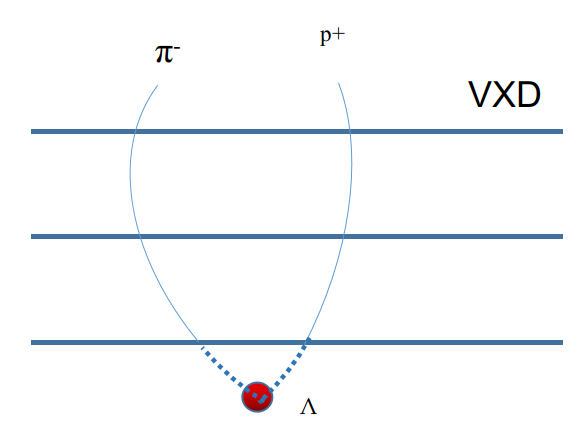
\includegraphics[width=7cm]{fakeks3} 
		\label{fig:side:a} 
	\end{minipage}%
	\begin{minipage}[t]{0.5\linewidth} 
		\centering 
		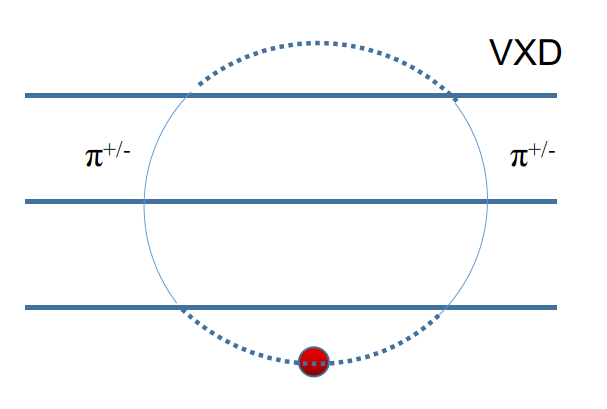
\includegraphics[width=7cm]{fakeks4} 
		%\caption{ } 
		\label{fig:side:b} 
	\end{minipage}% 
	
	\caption{The left shows the $\Lambda \to p^+ \pi^-$ decay shape that can be treated as $K_S^0$, the right shows a self-loop formed by a low $p_T$ charged pion reconstructed as two separated tracks with a vertex}
\end{figure}

\subsection{Determination of training observables from $K_S^0$ decay }
Given the characteristics of  $K_S^0 \to \pi^+ \pi^-$ discussed in the previous section, a set of observables as training features of FastBDT classifier can be constructed. The set includes categories of observables: kinematics, decay shape parameters , particle identifications and detector hits information. Observables are listed below with a sketch showing the shape parameters of $K_S^0$ decay in Fig 3-8. 

\begin{itemize}
	\item Kinematics
	\begin{itemize}
		\item Invariant mass of $K_S^0$ before and after fitting vertex
		\item momentum of $K_S^0$ and $\pi^{+/-}$, vectors and magnitudes. 
	\end{itemize}
	
	\item Decay shape parameters
	\begin{itemize}
		\item cosine angle between $K_S^0$ vertex and momentum.
		\item helicity angle of two daughters in reference of $K_S^0$ momentum.
		\item decay angle of two daughters in the mother's frame. 
		\item flight distance projection on $K_S^0$ momentum direction.
		\item significance of flight distance, defined by ratio of flight length and its uncertainties.
		\item distance on z-axis of two daughters helix 
		\item impact parameters on $K_S^0$ vertex
	\end{itemize}
	
	\item Particle identifications
	\begin{itemize}
		\item pion-ID for $K_S^0$ daughters.
		\item muon-ID for $K_S^0$ daughters.
		\item proton-ID for $K_S^0$ positive charged daughter. 
	\end{itemize}

	\item Hits information
	\begin{itemize}
		\item the number of PXD hits for each $K_S^0$ daughter, up to 2.
		\item the number of SVD hits for each $K_S^0$ daughter.
		%\item the number of CDC hits for each $K_S^0$ daughter. 
	\end{itemize}
	
\end{itemize}

\begin{figure}
	\centering
	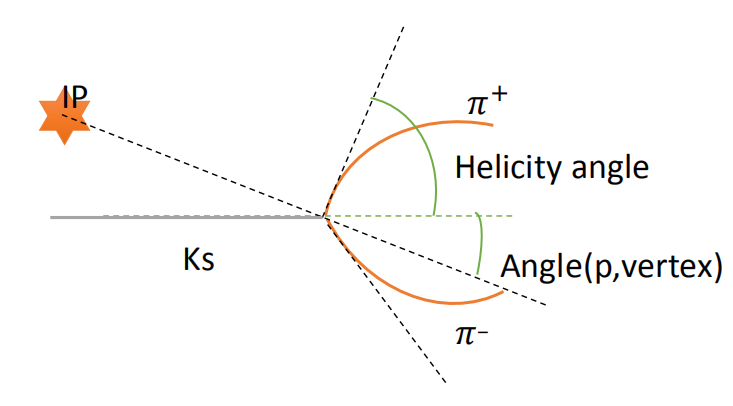
\includegraphics[height=6cm]{decayshape}
	\caption{The decay shape parameters, vertex vector takes IP as origin. }
\end{figure}


The decay shape category is of the most importance because it demonstrates the best separation power. For instance, if a false combination is made of two tracks, it's likely that the momentum direction of reconstructed fake $K_S^0$ is not aligned with the vertex position. So the projection of flight length on the momentum could be negative value for background. While in case of a true $K_S^0$, such projection is almost always a positive value.
 
There are a few points to be checked for using FastBDT classification, given the nature of the algorithm.
 First, the distribution of the observables should be different in true $K_S^0$ and background, so the FastBDT classifier can perform distinguish the true and the fake at each nodes to maximize the separation gain, just as Section 3.2.2 discussed. Secondly, there will a correlation among the training observables and they should also be different in signal and background. The boosting phase will create a sequence of shallow DTs whose structures are not same. Different correlations helps improve the performance of DTs in tuning of structure. For instance, a true $K_S^0$ flights longer by larger momentum in general, so its daughters' detector hits number becomes fewer. Then these two observables have negative correlations in true $K_S^0$. In case a fake $K_S^0$, the flight length could be a deep outside of VXD  but daughters may have full VXD hits, without clear correlation. At last, one should also avoid using many observables with too strong correlations since the classifier won't gain much improved separation power when put a cut on each of them. The correlation of the observables in signal and background samples are shown in Fig 3-9. The selected observables meets the requirements for classification. 
 
 \begin{figure}
 	\centering 
 	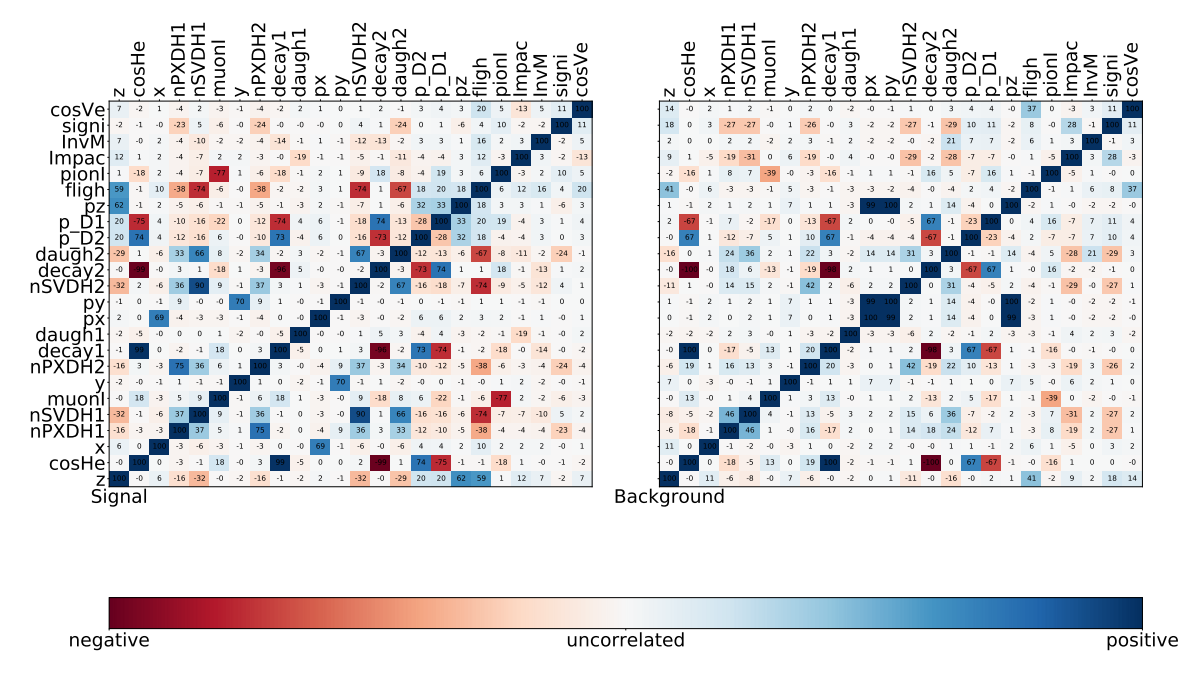
\includegraphics[height=8cm]{corks}
 	\caption{The correlation matrix of the chosen observables. It shows different correlation between observables in signal and background. And there's no single observable showing strong correlation with all other members. }
 \end{figure}
 

 \subsection{Training, Testing and Application of KsFinder}
 Training samples of $K_S^0$ are first extracted based on ``stdKshort:merged" from generic $B^0$ decay and $B^0 \to K_S^0  K_S^0  K_S^0$ using MC13 samples, respectively. For the hyper-[arameters of FastBDT method, the depth of each DT is 3 and the number of total trees (boosting steps) is 200, with a balance of computing time and performance. The training target variable is ``isSignal" flag. The ratio between the true and fake $K_S^0$ is 1:1 in both training and tesing sample. The training sample and tesing sample are separately prepared using different input file from MC13. The distribution of observables in true and fake samples (from $B^0 \to K_S^0  K_S^0  K_S^0$) are shown in the Appendix A. The abbreviations of those variables and their importance rank are shown in Table 3.2 and 3.3. 
 
 \begin{table} [ht]
 	\begin{minipage}[t]{0.5\linewidth}
 		\centering
 		\caption{The Abbreviations.}
 		\begin{tabular}{c|c}
 			\hline
 			Observables &  Abbreviations\\
 			\hline
 			nPXDHits\_D1 &  nPXDH1 \\
 			decayAngle\_D1 & decay1 \\
 			nPXDHits\_D2 & nPXDH2\\
 			y & y \\
 			decayAngle\_D2 & decay2\\
 			px & px\\
 			z & z \\
 			cosHelicityAngleMomentum & cosHe\\
 			x & x \\
 			daughtersDeltaZ & daugh1\\
 			nSVDHits\_D1 & nSVDH1\\
 			py & py\\
 			muonID\_pi & muonI\\
 			nSVDHits\_D2 & nSVDH2\\
 			p\_D1 & p\_D1\\
 			p\_D2 & p\_D2\\
 			pz & pz \\
 			flightDistance & fligh\\
 			pionID\_pi & pionI\\
 			InvM & InvM \\
 			daughterAngle2body & daugh2\\
 			ImpactXY & Impac \\
 			significanceOfDistance & signi \\
 			M & M \\
 			cosVertexMomentum & cosVe \\
 			\hline
 		\end{tabular}
 		\label{fig:side:a} 
 	\end{minipage}
 	\begin{minipage}[t]{0.5\linewidth}
 		\centering 
 		\caption{Importance rank }
 		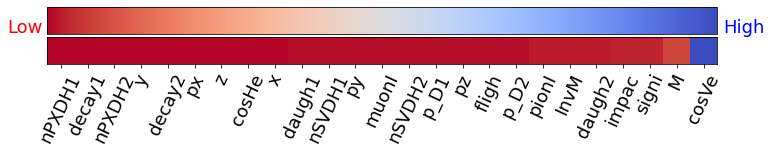
\includegraphics[width=4cm]{rank1}
 		\label{fig:side:b} 
 	\end{minipage}
 \end{table}

\subsection{The Performance and Over-fitting check}
The performance of classifier is evaluated by applying it on a independent data sample. So in the accordance of training data used, the same mount of events are prepared. Since the training is performed on three different types samples, three classifiers are actually obtained. Signal efficiency and background rejection are calculated using the output of trained classifier that presents the likelihood of probability of being a true $K_S^0$, as defined in Eq (3.1) and Eq (3.2).  

\begin{eqnarray}
	\text{signal efficency} = \frac{\text{Number of true $K_S^0$ with output $>$ cut value}}{\text{Number of all true $K_S^0$ }} \\
	\text{background rejection} = \frac{\text{Number of fake $K_S^0$ with output $<$ cut value}}{\text{Number of fake true $K_S^0$ }}
\end{eqnarray}

Using the weight file created by the training process, the output between 0 and 1 is assigned to every candidates as a quality index standing for the likelihood to be true $K_S^0$ that can be used as a cut. In order to check the performance of the classification, the ROC (receiver operating characteristics) curve is plotted, which shows the dependence of rejection power regarding the signal purity. The larger area a ROC curve is covered, meaning that background rejection drops slower when increasing classifier cut, the better performance is achieved. Three classifiers are tested with generic $B^0$ decay, and $B^0 \to K_S^0  K_S^0  K_S^0$ to check the robustness of classifier. The ROC, signal efficiency and purity are shown: 

\begin{figure}[H]
	\begin{minipage}[b]{0.5\linewidth}
		\centering 
		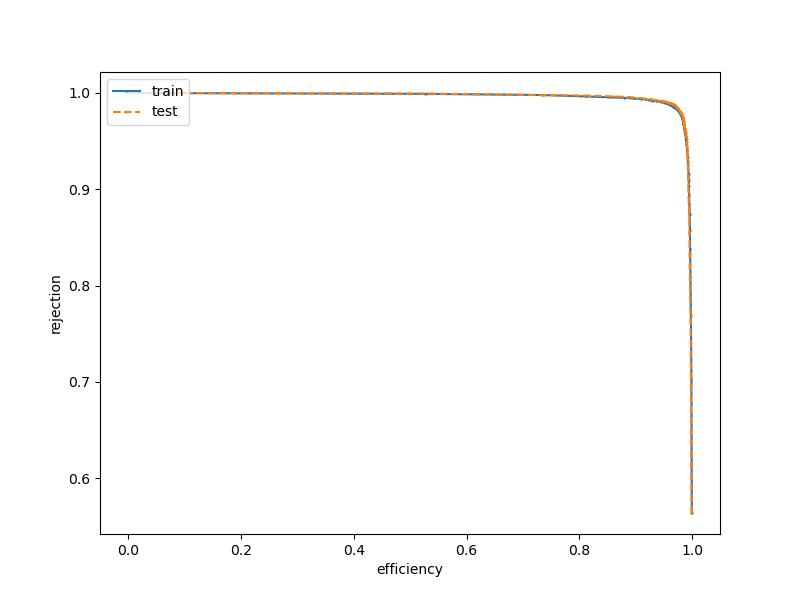
\includegraphics[height=6cm]{ROC_3Ks}
		\label{fig:side:a}
	\end{minipage}
	\begin{minipage}[b]{0.5\linewidth}
		\centering 
		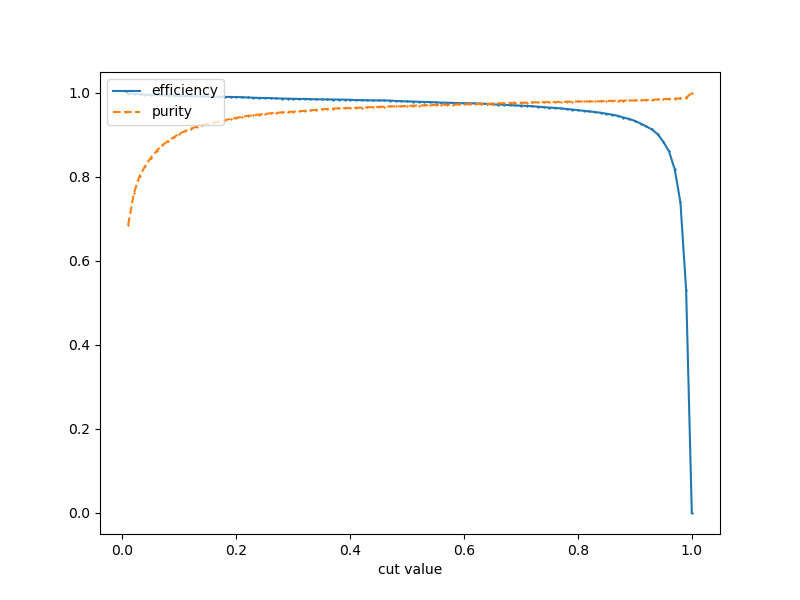
\includegraphics[height=6cm]{eff_3Ks}
		\label{fig:side:b}
	\end{minipage}
\caption{The left is ROC curve(blue for training and orange for testing) and the right is efficiency and purity (blue for efficiency and orange for purity) depending on cut of classifier output. Results are from $B^0 \to K_S^0  K_S^0  K_S^0$ sample.}
\end{figure}

\begin{figure}[H]
	\begin{minipage}[b]{0.5\linewidth}
		\centering 
		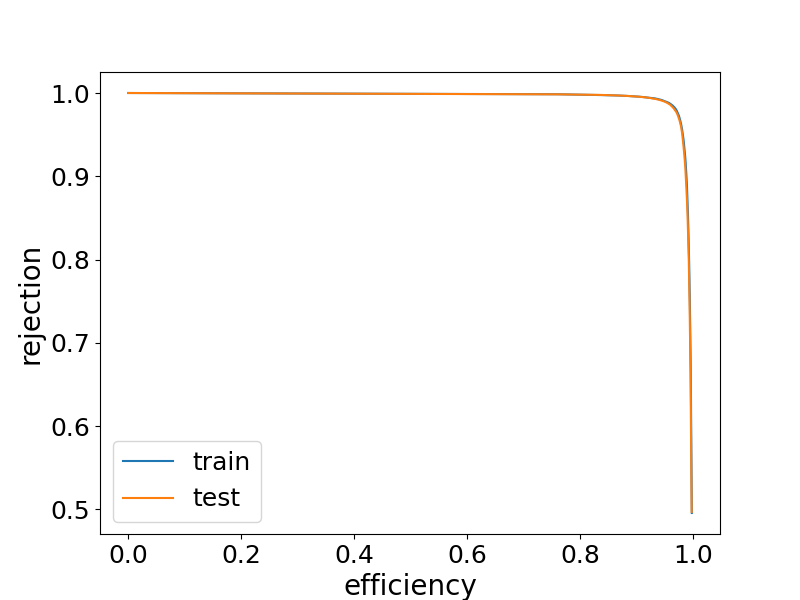
\includegraphics[height=6cm]{ROC_gen}
		\label{fig:side:a}
	\end{minipage}
	\begin{minipage}[b]{0.5\linewidth}
		\centering 
		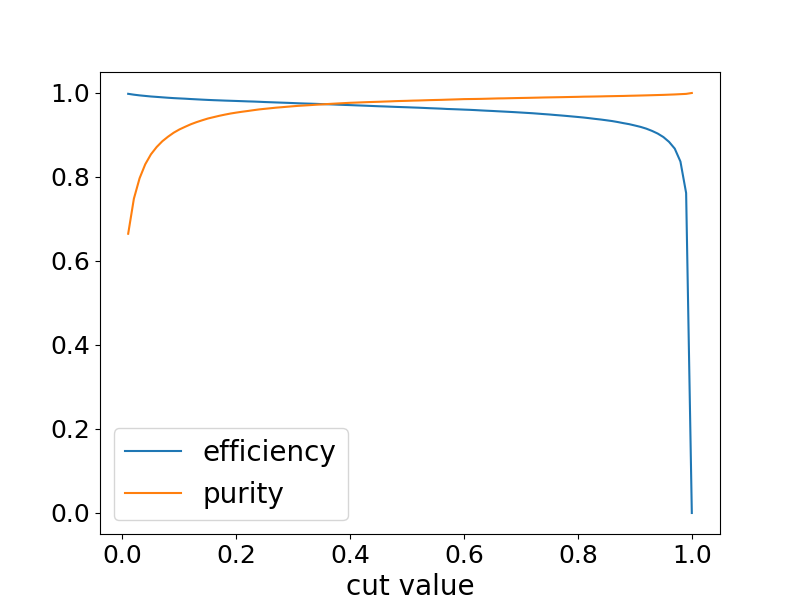
\includegraphics[height=6cm]{eff_gen}
		\label{fig:side:b}
	\end{minipage}
	\caption{The left is ROC curve (blue for training and orange for testing) and the right is efficiency and purity (blue for efficiency and orange for purity) depending on cut of classifier output. Results are from $B^0$ generic decay sample.}
\end{figure}

\begin{comment}
\begin{figure}[H]
	\begin{minipage}[b]{0.5\linewidth}
		\centering 
		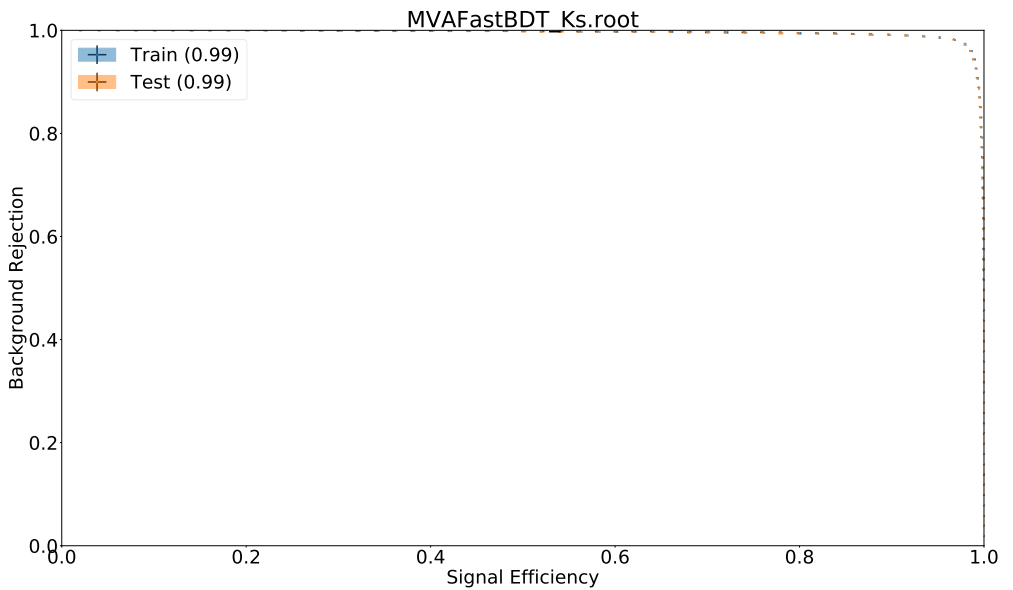
\includegraphics[height=4cm]{jpsi-jpsi}
		\label{fig:side:a}
	\end{minipage}
	\begin{minipage}[b]{0.5\linewidth}
		\centering 
		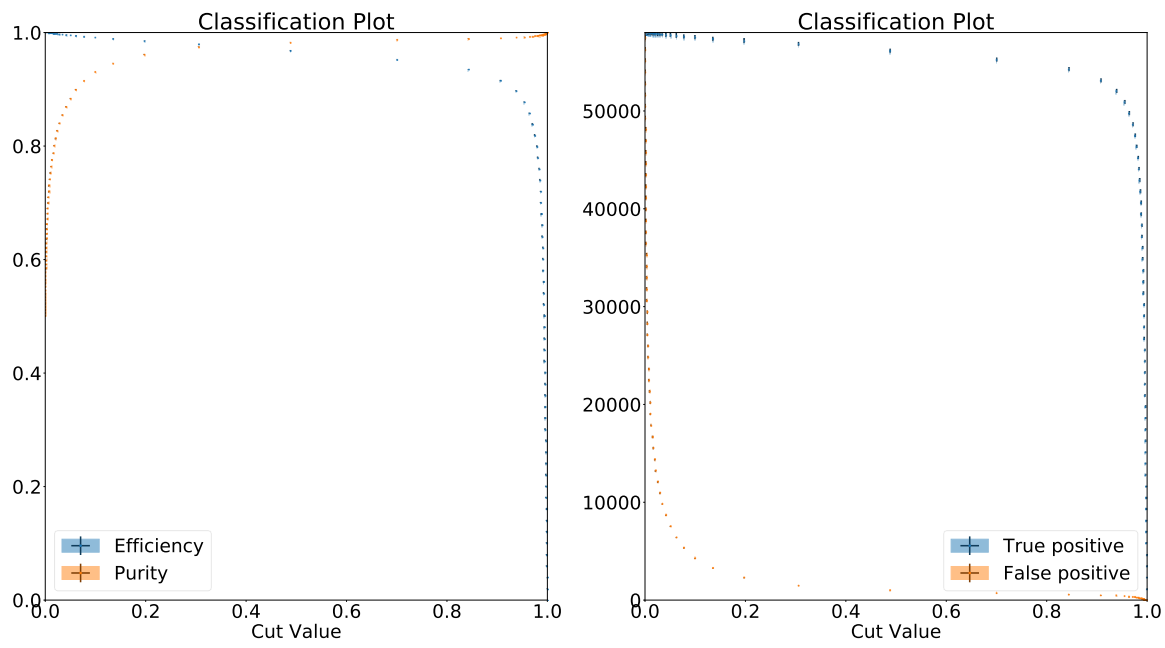
\includegraphics[height=4cm]{jpsi-jpsi-pur}
		\label{fig:side:b}
	\end{minipage}
	\caption{The left is ROC curve and the right is efficiency and purity depending on cut of classifier output. Results are from $B^0 \to J/\psi K_S^0$ generic decay sample.}
\end{figure}
\end{comment}


The ROC curves show a good rejection power on classifiers. To be noted, the curves are consistent in training and testing samples. 
While the ROC curve has shown the absence of noticeable over-fitting in classification, the detailed check can be made by comparing the distribution of classifier output on true and fake $K_S^0$ respectively in training and testing. In the classifiers we obtained, results from training and testing are very much close thus no over-fitting is spotted, as shown in Fig 3-13.
\begin{figure}[H]
	\begin{subfigure}{1\linewidth}
		\centering
		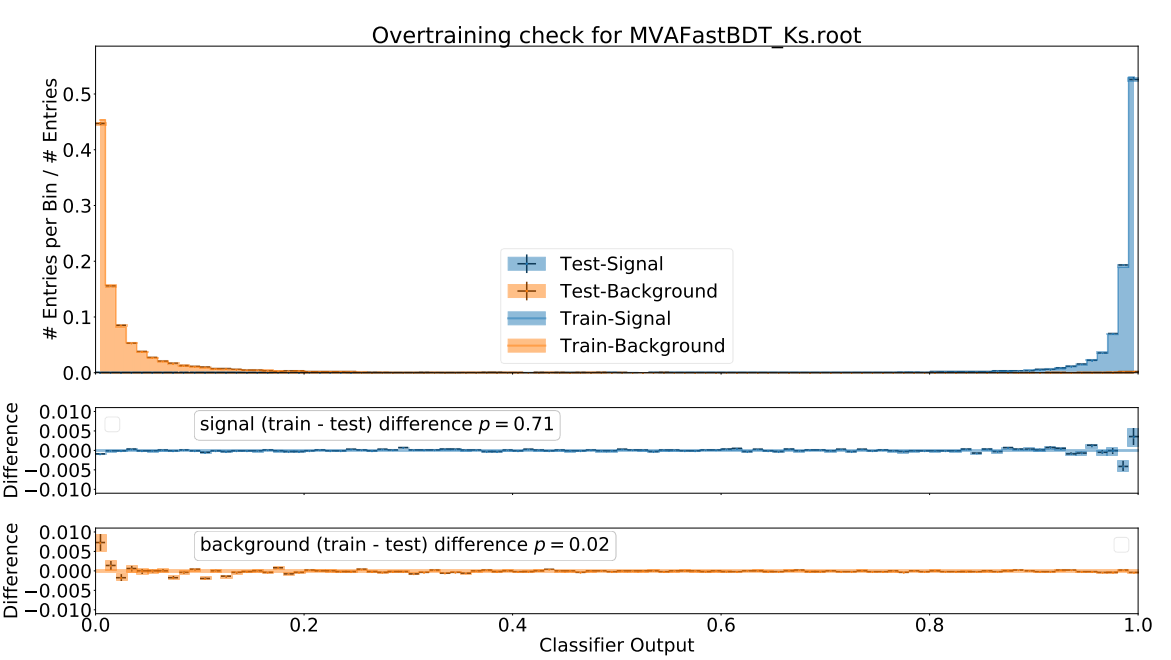
\includegraphics[height=6cm]{over-3ks}
		\caption{Over-fitting check for $B^0 \to K_S^0  K_S^0  K_S^0$.}
	\end{subfigure}
  	\vspace{0.3cm}

	\begin{subfigure}{1\linewidth}
		\centering
		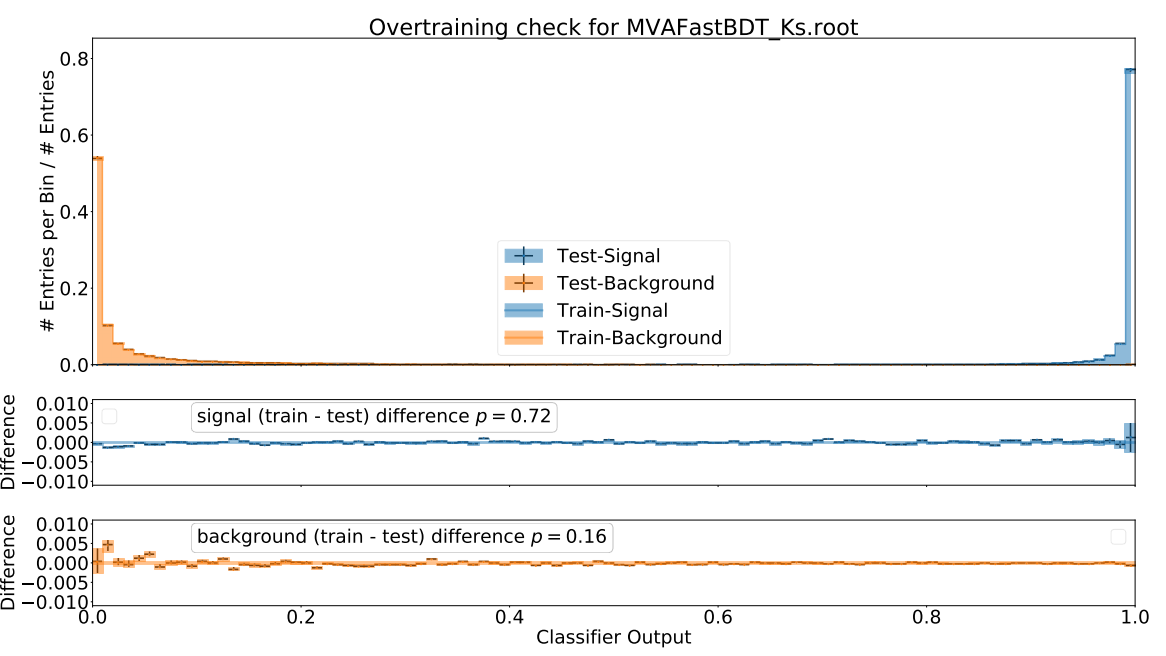
\includegraphics[height=6cm]{over-gen}
		\caption{Over-fitting check for $B^0$ generic decay.}
	\end{subfigure}
	\vspace{0.3cm}
	
%	\begin{subfigure}{1\linewidth}
%		\centering
%		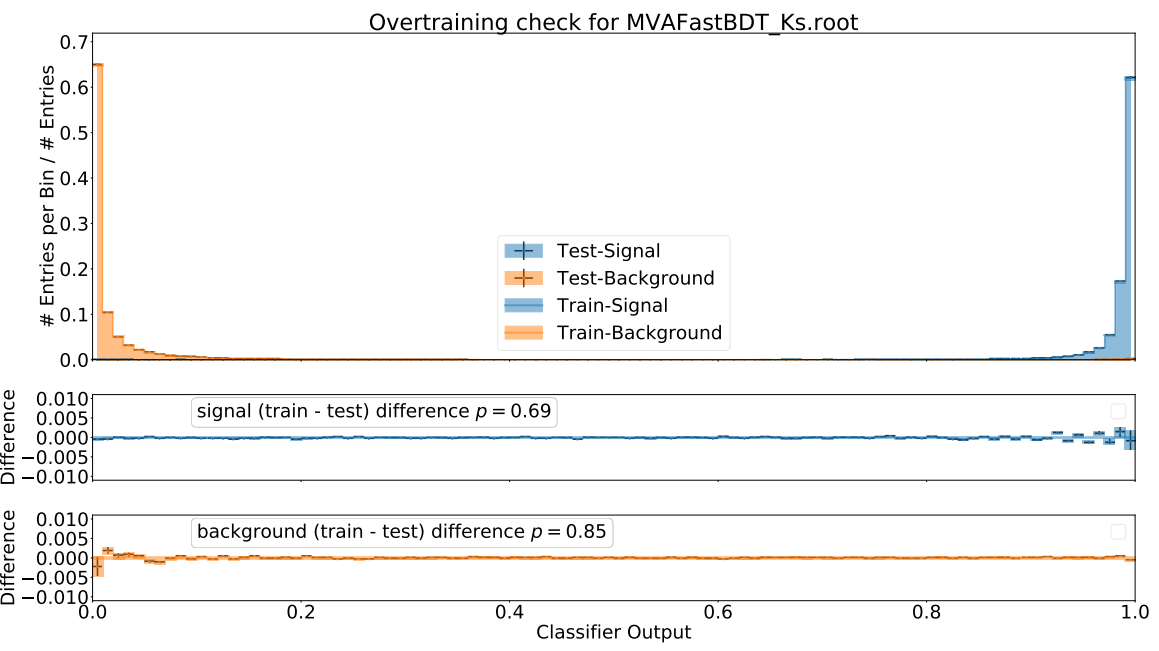
\includegraphics[height=6cm]{over-jpsi}
%		\caption{Over-fitting check for  $B^0 \to J/\psi K_S^0$.}
%	\end{subfigure}
%\caption{Over-fitting check for classifiers.}
\end{figure}

In order to use the output of KsFinder, a cut value must be chosen. The output of KsFinder is named ``FBDT\_Ks". Here we can define a ``Figure of Merit" (FOM) to determine the cut value. S and B is the number of true and fake $K_S^0$ after the cut,respectively. The value of 0.74 of ``FBDT\_Ks" maximize the KsFinder output in $B^0 \to K_S^0  K_S^0  K_S^0$, so we will use this value as only $K_S^0$ with larger ``FBDT\_Ks" will be kept from cut-based selection.

\begin{equation}
	\text{FOM} = \frac{S}{\sqrt{S+B}}
\end{equation}

\begin{figure}[H]
	\centering
	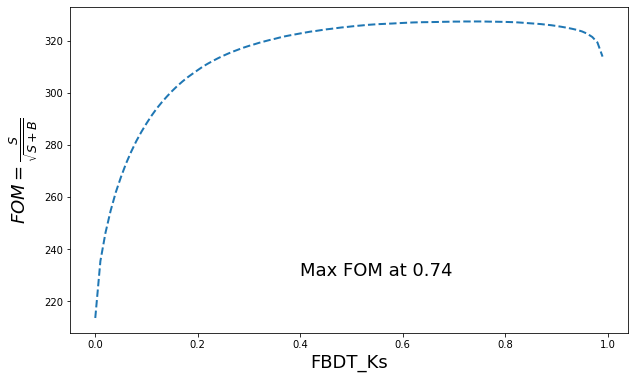
\includegraphics[width=0.6\linewidth]{fom3ks}
	\caption{FOM of classifier output (FBDT\_Ks) in $B^0 \to K_S^0  K_S^0  K_S^0$, maximum value is obtained at 0.74 and curve is almost flat after 0.5.}
\end{figure}

By comparing the fitted invariant mass of $K_S^0$ before and after the application of this cut, it's clear that the fraction of background has been largely reduced and most of the signal remains. The true $K_S^0$ fraction in the pre-selected $K_S^0$ before applying KsFinder cut is 39\%, and 95.3\% of them are remained after KsFinder applied. The fake $K_S^0$ fraction before applying KsFinder cut is 61\%, and 97.6\% of them are rejected after KsFinder applied. A much cleaner $K_S^0$ candidates is created as shown in Fig 3-15. 

\begin{figure}[htpb]
	\centering
	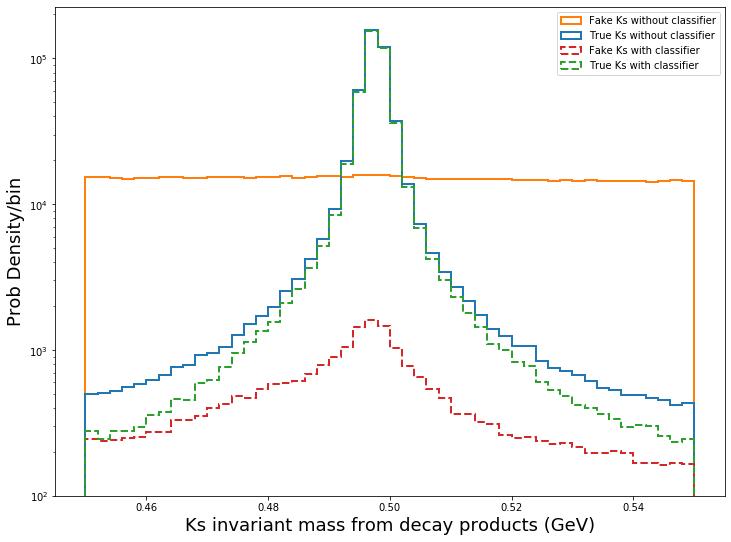
\includegraphics[width=0.8\linewidth]{kscutM}
	\caption{$K_S^0$ purity improvement with cut value of FBDT\_Ks at 0.74 applied. Blue solid line is true $K_S^0$ before KsFinder and green dashed line is the true $K_S^0$ after. The orange solid line is fake $K_S^0$ before KsFinder and red dashed line is fake $K_S^0$ after. 95.3\% of true $K_S^0$ are kept while 97.6\% the fake are rejected by the classification. }
\end{figure}

\subsection{Data Validation for Classifier}
The results from MC studies show an excellentperformance of KsFinder. However, such classification is based on the observables reconstructed from MC samples, and FastBDT algorithm is depending on the training features apparently. As a result, the validation of such tool on the real experiment data is necessary. This would justify the usage of classifier on data and is also essentially helpful to check the potential discrepancy between MC and data. 

The validation comes from the following aspects. First of all, since there's no ``isSignal" truth in real data, there's no way to direct check performance on data. Since the FastBDT method is based on the distribution of training variables, if these variables shows close distribution among MC and data, then the classification performance is expected to be close.

 Thus, variables must be compared between data and MC to ensure the consistence. Then, the expected performance represented by the distribution of selected $K_S^0$ should be similar between data and MC. Particularly, since $K_S^0$ candidates will be used for further reconstruction of $B^0$, its kinematics such mass and momentum may change after the classifier application, so the validation that approves no clear bias on $B^0$'s $M_{bc}$ and $\Delta E$ which are used for $B^0$ reconstruction is also needed.

We take the small data sample from Belle II early phase 3 operation experiment 7 and 8 in 2019 for comparison. The integral luminosity at $\Upsilon(4S)$ resonance is about 5.17 $\text{fb}^{-1}$.  MC13 sample is extracted from generic $B^0$ decay with equivalent events number. There are two campaigns of MC included (MC12b and MC13, later one is the latest). Fig 3-16 shows the invariant mass and momentum distributions from data and MC samples, and full comparison of all training variables is included in Appendix B. Most of the distribution shows a good consistence before and after using KsFinder. It shows that kinematics of $K_S^0$ in data and MC yield fairly close distributions and no clear bias is seen by applying the KsFinder cut.

\begin{figure}[H]
	\begin{subfigure}{0.5\linewidth}
		\includegraphics[page=2,height=4cm]{dataVarsPlot_Ks.pdf}
	\end{subfigure}
	\begin{subfigure}{0.5\linewidth}
		\includegraphics[page=7,height=4cm]{dataVarsPlot_Ks.pdf}
	\end{subfigure}
	\bigskip
	\begin{subfigure}{0.5\linewidth}
		\includegraphics[page=8,height=4cm]{dataVarsPlot_Ks.pdf}
	\end{subfigure}
	\begin{subfigure}{0.5\linewidth}
		\includegraphics[page=9,height=4cm]{dataVarsPlot_Ks.pdf}
	\end{subfigure}
\caption{The distribution of invariant mass from daughters and the momentum of x,y,z direction. Blue bar is from all MC13, cyan bar is the true $K_S^0$ in it. Yellow step histogram is data with no cut, solid red data with MC13 trained cut, and the dashed is with MC12b cut. Experimental data has a good agreement with MC before and after applying the KsFinder.}
\end{figure}

\subsection{KsFinder Effects on Kinematics Evaluation}
Implementing KsFinder for $K_S^0$ may induce extra bias on the event numbers for $K_S^0$. It's not easy to direct evaluate the impact of each variables in training towards the final signal yield because the output is non-linear dependence on those variables. However, we can directly use the output of KsFinder and introduce the scale factor when check the data and MC signal yields. 
 
A fit on invariant mass $M$ of $K_S^0$ candidates after varied cut on KsFinder output is done by modeling signal shape as double-Gaussian and background as Chebyshev polynomial. Significance is define as $S_{data/MC} = N_{signal} /N_total$ in data and MC from fitting using RooFit. A list of intervals of cut value on KsFinder output is made and the significance is calculated within each interval. Fitting results are shown in Fig 3.17 using loose and tight cut respectively. The fit plots in all cut intervals are included in Appendix C.  Data/MC correction is defined as:

\begin{equation}
	R = \frac{S_{MC}}{S_{data}}
\end{equation}



\begin{figure}[htpb]
	\begin{subfigure}{0.5\linewidth}
		\caption{Data,cut=0.2}
		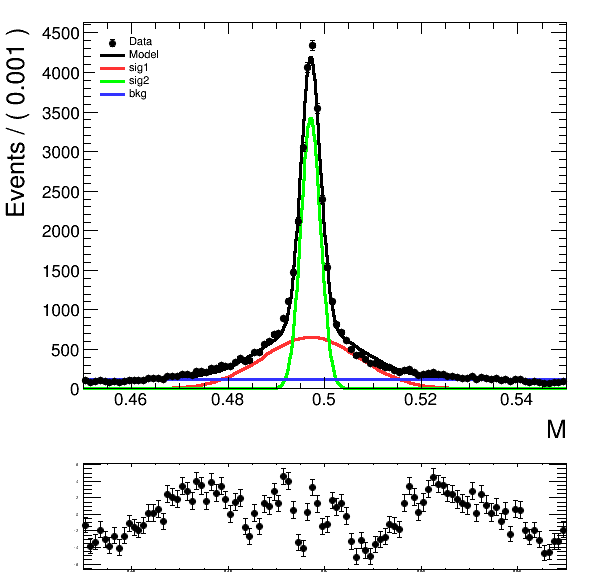
\includegraphics[width=1\linewidth]{ksDatamva0.2.png}
	\end{subfigure}
\begin{subfigure}{0.5\linewidth}
	\caption{MC,cut=0.2}
	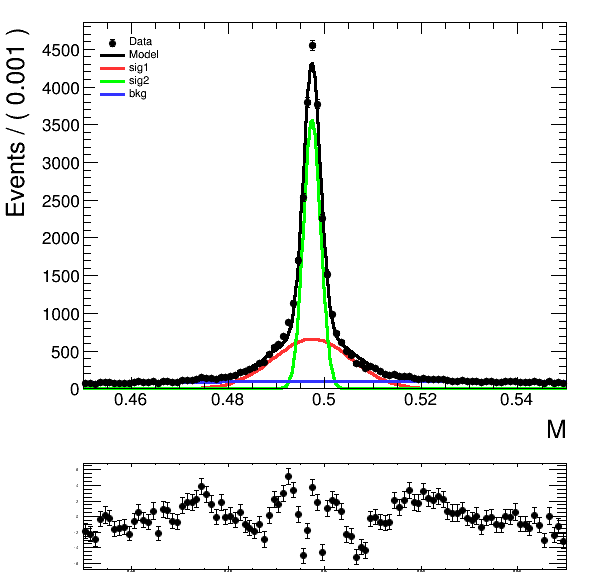
\includegraphics[width=1\linewidth]{ksMCmva0.2.png}
\end{subfigure}

\begin{subfigure}{0.5\linewidth}
	\caption{Data,cut=0.9}
	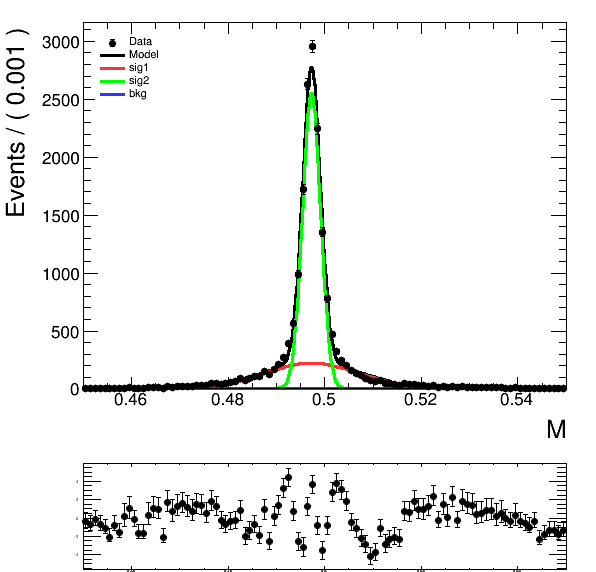
\includegraphics[width=1\linewidth]{ksDatamva0.9.png}
\end{subfigure}
\begin{subfigure}{0.5\linewidth}
	\caption{MC,cut=0.9}
	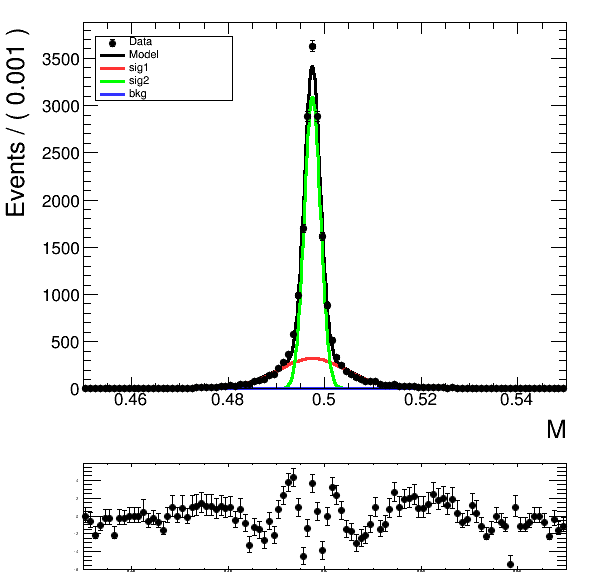
\includegraphics[width=1\linewidth]{ksMCmva0.9.png}
\end{subfigure}
\caption{Invariant mass fit of $K_S^0$ using cut at 0.2(loose) and 0.9(tight) to calculate $S_{data/MC}$.}
\end{figure}

The correction is defined by taking the R value within the chosen interval. Uncertainty of R is defined by the difference of maximum and minimum of R in all intervals. R is distributed as: 
\begin{figure}[H]
	\centering 
	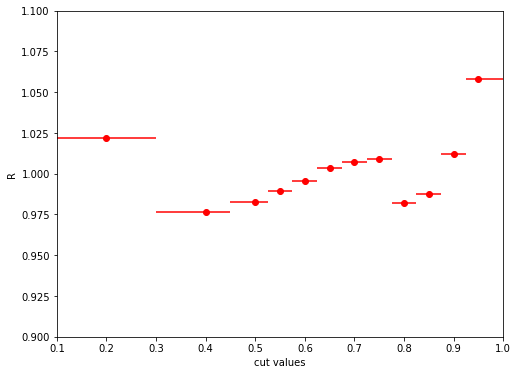
\includegraphics[width=0.7\linewidth]{Rc}
	\caption{Data MC correction induced by $K_S^0$ classifier.}
\end{figure}

The R, for example in cut value 0.74 of maximum FOM, is $R = 1.009\pm 0.081$. In $B^0 \to K_S^0  K_S^0  K_S^0$, the correction of $B^0$ events should be proportional to R to the three.  Correction that is implemented for $B^0$ is $1.027^{+0.33}_{-0.18}$. In most of the cut intervals, the R is within 2.5\% so the bias on $K_S^0$ numbers is very small.
\subsection{Summary}
The development of Belle II $K_S^0$ classifier is enlighten by the experience from Belle. A comprehensive study of training observables from $K_S^0$ decay characteristics has been exploited. It takes the advantage of FastBDT algorithm to achieve a high fake rejection power. As a result, classifier is able to give a output which can be used as a cut to select good $K_S^0$ candidates with high purity. The classifier is validated with real experimental data as well. A primary data validation study of KsFinder is conducted with implementing correction on data and MC along with its contribution to $B^0$. The performance of KsFinder is in a good shape and no clear bias is found on the yield of the number of $K_S^0$. For the reconstruction of $B^0 \to K_S^0  K_S^0  K_S^0$, the development of KsFinder is critical to suppress large fraction of combination background from fake $K_S^0$.

